\chapter{Introduction}
\label{chap:introduction}
\section{Motivation and Background}
Different renewable energy alternatives are being explored as the world strives towards greener energy.  Man has utilized wind for thousands of years, and in recent years, wind energy has become one of the more mature renewable energies. As the areas on land that are fit for wind turbines are limited, and the public is dissatisfied with the noise and visibility of the wind turbines, technology is advancing towards offshore wind parks. Moving the wind parks offshore is not only solving the problems with criticisms from the public, but wind speed tends to increase with distance from shore. In the last years, there has been an increase in scale, capacity, and distance from shore each year for offshore wind installations. Moving further from shore often implies moving into deeper waters, making floating wind turbines the most plausible technology.\\\\ Floating wind turbines are similar to semi-submersible oil platforms, but have very different motions, as geometry and wind loads are significantly different. Extensive research has been done in terms of evaluating the lifetime for flexible risers and umbilicals in relation to fatigue for the oil and gas industry. For floating wind turbines, there is considerably less research done in terms of the lifetime of dynamic flexible cables. As the power cables that are connected to floating structures are subjected to oscillations due to movements of the vessel in waves, fatigue strength requires to be verified for design.\\\\ A conductor usually consists of several conductors with layers of copper wires in each conductor. The wires are stranded helically around a core wire, and this causes contact both between the conductors, and between each layer in the conductors. The complex contact situation makes the cable vulnerable for fretting fatigue in addition to fatigue due to the cyclic variation in curvature and tension due to the vessels movements in the waves,  \cite{s300}. \cite{Karlsen2010} clarifies that neither the fatigue properties, nor the methods to ascertain SN-data of copper conductors are established by the cable or offshore industry.  Knowledge about power cable technology and the lifetime of power cables is one of the most important limiting factors of moving wind floating wind turbines further away from shore and into deeper waters. To continue the advancement of floating wind turbines in the future, research is necessitated, \cite{Thies2012}.
\newline
\newline
Lifes50+ is a project funded by the Horizon2020 program where the purpose is to develop cost-effective floating solutions for 10MW wind turbines, \cite{Horizon2010}. The project consists of 4 different designs and 3 separate locations. One of the designs in the project is the OO-Star developed by Dr. Techn. Olav Olsen shown in Figure \ref{fig:oostarintro}. OO-Star was deemed an appropriate base for a case study to review the lifetime of dynamic power cables further.

\begin{figure}[H]
\centering
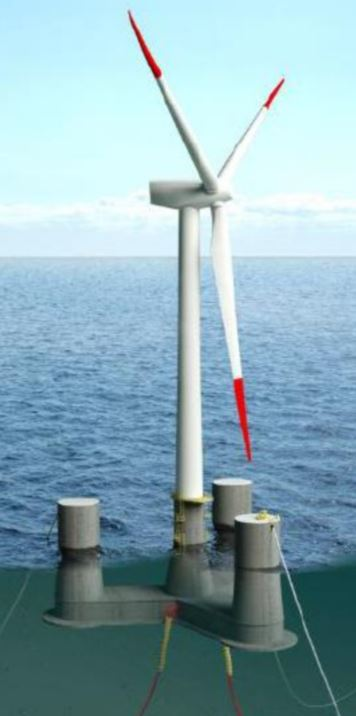
\includegraphics[scale=0.5]{figures/oostar}
\caption[$\; \:$Dr. Techn. Olav Olsen's OO-Star]{Dr. Techn. Olav Olsen's OO-Star \cite{Lifes50+D4.2} }
 \label{fig:oostarintro}
\end{figure}


\section{Literature Review}
A literature search was done prior to the project thesis. \cite{Feld1995} looked at the applied loads and responses of the metallic elements for subsea configurations. \cite{Alani1997Eoma} studied the effect of mean axial load on axial fatigue life of spiral strands, and concluded that increasing lay angle had a significant negative effect on endurance limit for both the outer and wires in a spiral strand. \cite{Chien2004} discussed different cable designs for 250MW offshore power transmission and concluded that they do not behave like umbilicals dynamically, and that harmonics do occur during transmission. \cite{Raoof2008} looked at axial fatigue design of sheathed spiral strands in deepwater applications, and concluded that (among other things) that the fatigue life of stranded spirals is significantly shorter at the end termination than in free-field. \cite{Karlsen2010} presented a test method for simulating fatigue of a dynamic power cable that included the effects of fretting, creep and friction.\\\\ \cite{Nasution2013} investigated fatigue on 95mm$^2$ copper conductors experimentally and by the use of FEM. Single wires from different layers were tested in tension, and the full cross-section was tested in bending. The full cross-section showed lower fatigue strength that the individual wires and trellis points were particularly vulnerable, as cracks initiated from these points. It was suggested that the difference in results between the testing and the FEM analyses was due to the surface irregularities in the wires from the packaging of the conductor. \cite{NASUTION2014} did similar tests and concluded that all first fatigue failures in tension-tension of the full cross-section happened in the outer layers of the conductors, in the thinnest parts of the wires, that is, the trellis points. For tension-bending mode, all the failures occurred in the inner layer of the conductor. It was concluded that this indicated that the effect of friction between layers plays an important role in the lifetime of the cross-section. The report also comments that as the longitudinal stress governs the fatigue performance, beam elements can be used with good results in analyses. \cite{s300} did experimental and FEM analysis of fatigue strength with 300mm$^2$ conductors. This study concluded with that in terms of maximum stress, individual wires from 95mm$^2$  and 300mm$^2$ wires fall in a common scatter band, and that lubricated conductors have longer fatigue life than unlubricated conductors. The study also supports the previous conclusions that crack initiation starts from trellis points. In this article, an analytic method to calculate the stress variation in the individual wires of the conductor was developed. \cite{Taninok2017} looked at dynamic cable systems for 2MW and 100kW floating offshore wind installations and concluded that their proposed cable profile absorbed the floater behavior so that there was no motion in the cable at the bottom hang off.  

\section{State of the Art}
\subsection{Offshore Wind Turbines}
According to ISSC 2018 committee V.4: OFFSHORE RENEWABLE ENERGY: (\cite{Gao2018}): "Offshore wind is by far the most developed technology and
promising cost reduction has been achieved in the last few years," in terms of offshore renewable technologies. Figure \ref{fig:sit17} shows the development of offshore wind capacity until 2017. 

\begin{figure}[H]
\centering
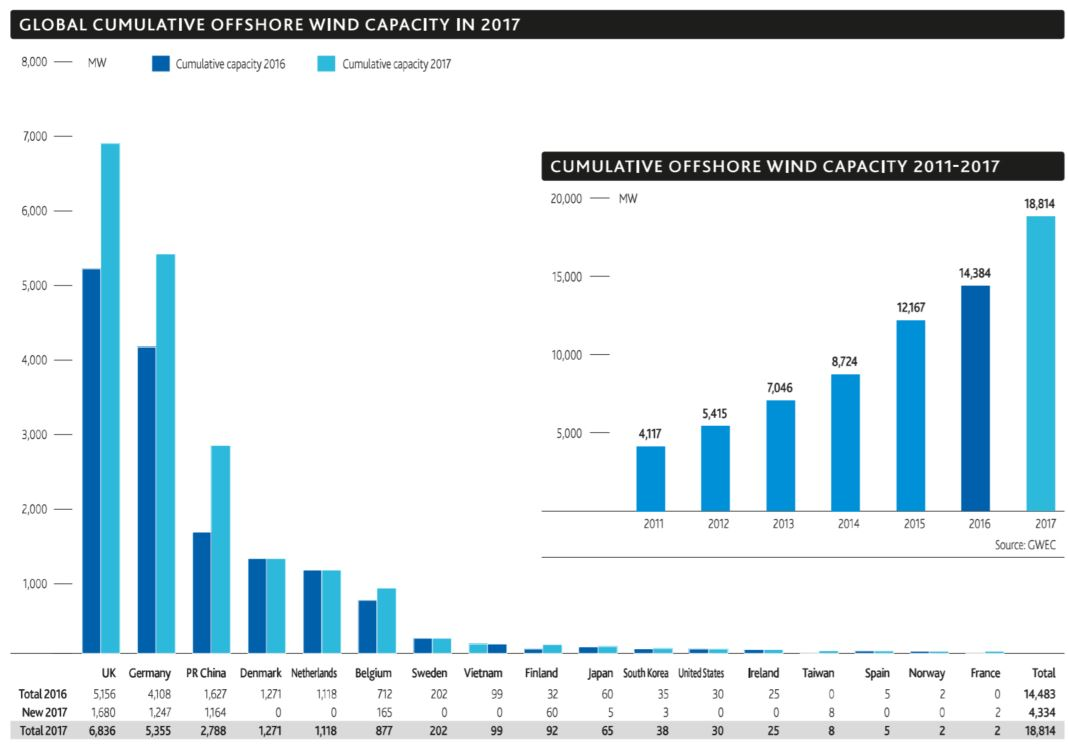
\includegraphics[scale=0.8]{figures/sit17}
\caption[$\; \:$Cumulative Offshore Wind Capacity in 2017]{Cumulative Offshore Wind Capacity in 2017 \cite{GWEC2018}}
 \label{fig:sit17}
\end{figure}

\noindent The majority of the offshore wind farms are located in Europe. Figure \ref{fig:world} presents the current market situation of offshore floating wind turbines. As can be seen, it is mainly Europe, the USA, and China that are represented. 


\begin{figure}[H]
\centering
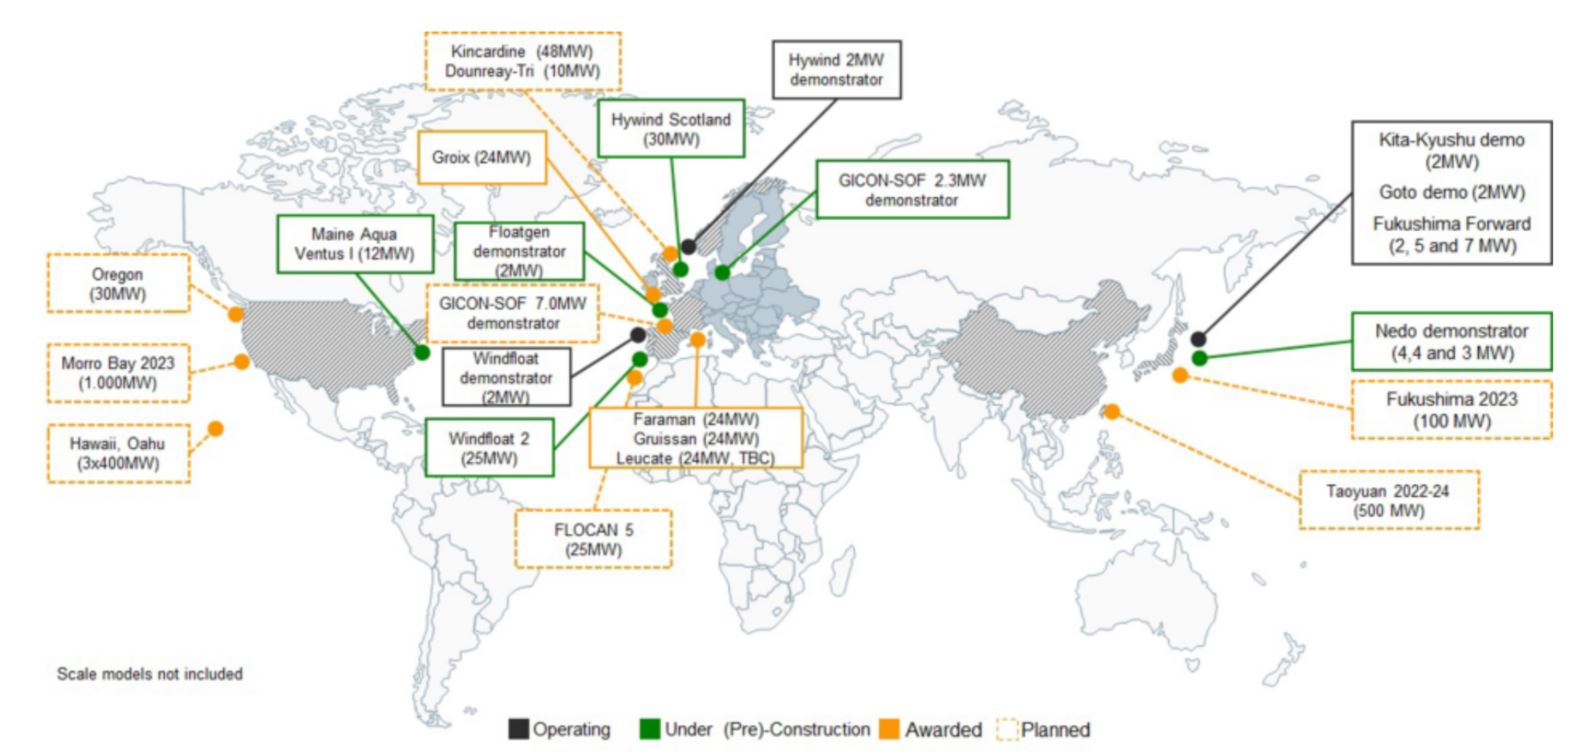
\includegraphics[scale=0.54]{figures/world}
\caption[$\; \:$Current market situation of offshore floating wind turbines]{Current market situation of offshore floating wind turbines \cite{Gao2018}}
 \label{fig:world}
\end{figure}

\noindent In recent years, installations have moved further from shore, into deeper waters and with large farm configurations and larger turbines.  Longer blades give advantages in terms of overall cost, but also challenges for installation, \cite{Gao2018}.  Figure \ref{fig:diameter} shows the development of power capacity for the last two centuries. The average size in 2017 was 5.9 MW. That is an increase of 23\% from 2016, according to \cite{we2018}.

\begin{figure}[H]
\centering
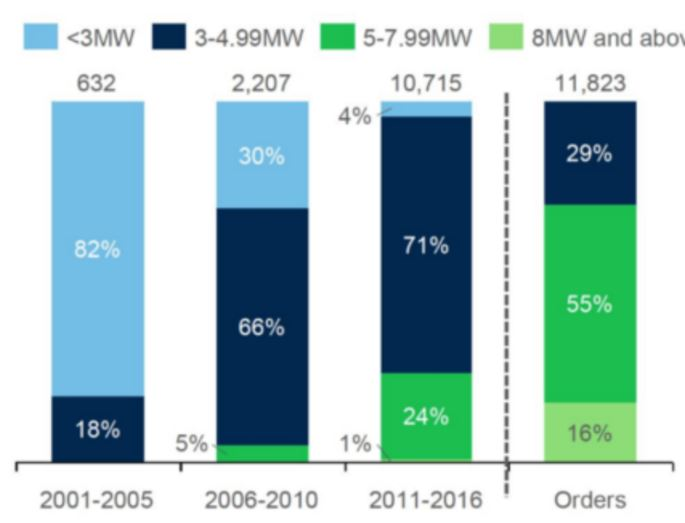
\includegraphics[scale=0.7]{figures/diameter}
\caption[$\; \:$Development of turbine size]{Development of turbine size. \cite{Deigen2018}}
 \label{fig:diameter}
\end{figure}

 \noindent In 2016, the first 8 MW turbine was installed in the Irish Sea in the UK. In Norway, Statoil made a step towards commercialization of floating wind farms by installing the first floating wind farm with 5 6MW spar wind turbines called Hywind, outside of Scotland. Hywind can be employed at depths up to 800m, and enable offshore wind energy installations for areas that have been unavailable until now \cite{Equinor2018}. Short-term plans for the offshore wind industry cover the installation of two small floating wind farms in the US as well as prototype testing for exiting prototypes in Norway, Portugal, and Japan, and planned prototype development in Japan, France, and Germany.  Two large wind farms are projected on the east coast of the US, one 120 MW farm outside of Maryland, and one 90 MW on the coast of New York. \cite{Gao2018}. \newline
 \newline
 \cite{Bailey2014} states that "Commercialization of floating wind farms is
anticipated between 2020 and 2025." In 2014 the European Union set a legally binding target that 27\% of the energy consumption is to come from renewable energy sources in 2030. \cite{EWEA2015}  presents three separate scenarios on the development of offshore wind energy by 2030. The central scenario proposes that 66 GW  should come from offshore wind. To achieve this goal, an annual average increase of 15\% is required. \cite{Gao2018} states that the goal is probably reasonable as we have seen an increase of 25\%-30\% annually in recent years. US Department of Energy has a goal of 86 GW of energy provided from offshore wind by 2050, \cite{windus2016}. 
\subsection{Power Cables}
The trend over the years has been that offshore wind installations move further away from shore. This development is demonstrated in Figure \ref{fig:distshore}. 

\begin{figure}[H]
\centering
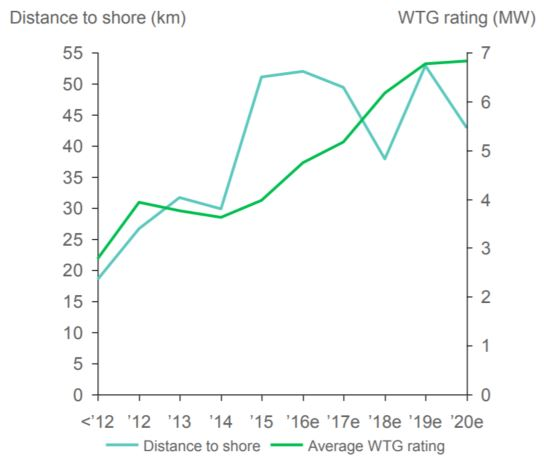
\includegraphics[scale=0.9]{figures/distshore}
\caption[$\; \:$Distance to shore ]{How distance to shore have increased in recent years \cite{Make2016}}
 \label{fig:distshore}
\end{figure}

\noindent \cite{srinil2016} states that traditionally, the w shape configuration has been used for inter-array cabling, and the lazy wave has been used for export cables, see Figure \ref{fig:cableconfig}. However, according to \cite{ds2010}, the lazy wave configuration is being considered for inter-array in newer projects such as the Statoil's Hywind project, and the Fukushima Floating Offshore Wind
Farm Demonstration Project, \cite{yagihashi2015dynamic}. Inter-array cables are usually three-core copper conductors, armored with steel wires with insulation around the conductors, \cite{srinil2016}. 


\begin{figure}[H]
\subfloat[Traditional W-shape for inter array cable \label{fig:dc}]
  {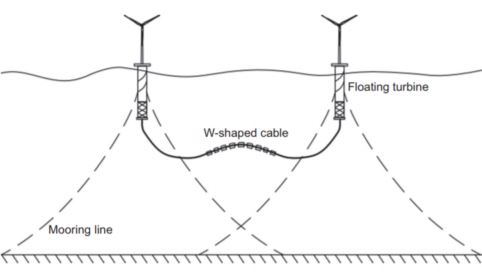
\includegraphics[width=.45\linewidth]{figures/wshape}}\hfill
\subfloat[Lazy wave shape, traditionally only used for export cables \label{fig:ac}]
  {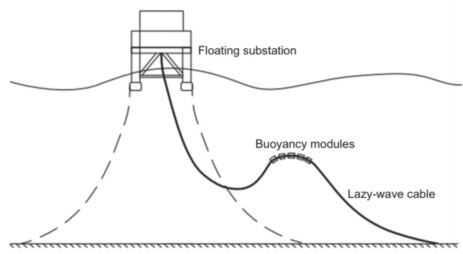
\includegraphics[width=.45\linewidth]{figures/lw}}\hfill
\caption[$\; \:$Cable configurations]{Different cable configurations, \cite{ds2010}}
\label{fig:cableconfig}
\end{figure}

\section{Objective}
The objective of this master thesis is to estimate the lifetime of a dynamic power cable applied in offshore wind farms.  Theory and software used and developed for the oil and gas industry, are implemented in the relatively new and upcoming field of ocean renewable energy.\\\\
The focus of this study is to estimate the fatigue life of a dynamic power cable at a chosen location through global and local analyses, and with the use of well-known fatigue calculation methods such as Rainflow counting, SN-curve, and Miner-Palmgren.  Besides, the study focuses on getting an insight into the mechanisms affecting the fatigue life of the cable down to fiber level in the power conductors. \\\\
This master thesis is a continuation of a project thesis that was completed in the fall of 2018.\\\\
The main objectives of this study are based on the Master Description attached earlier in this report. However,  several challenges were encountered as the study was conducted, and all choices or adjustments to the initial plan were made in close dialogue with the supervisor for the project, Professor Svein Sævik. The main objectives are:
\begin{enumerate}
    \item Perform a literature study and acquire the necessary theoretical background on all topics relevant for the master thesis, including but not limited to global and local analyses, offshore wind turbines, cable technology, and fatigue.
    \item Choose and establish a case scenario regarding wind turbine floater design, location, environmental conditions, cable design, and SN-fatigue data
    \item Create a global model in SIMA RIFLEX and determine cable configuration. 
    \item Create a local model in Bflex
    \item Perform global and local analyses and process the results to estimate the fatigue life of the dynamic power cable.
    \item Conduct a sensitivity study to investigate the friction mechanism in the conductor.  
\end{enumerate} 

\section{Contribution}
The main contribution from this study is the investigation of fatigue life of a dynamic power cable down to fiber level. By including calculation of friction effects on two levels, insight was gained on what affects the fatigue life of stranded helical copper conductors, whose fatigue properties are not well established. The fatigue life of dynamic power cables was examined by performing global and local analyses on a designated case scenario. The most important conclusion in this study is that contact between conductors, and between layers in each conductor contributes significantly to the fatigue damage, and should be included in analyses in the future. 
\section{Master Thesis Structure}
\begin{itemize}
    \item \textbf{Chapter 1} contains the introduction with a literature review, state of the art and objective for the master thesis.
     \item \textbf{Chapter 2} demonstrates the system theory for wind turbines, offshore wind turbines, and power cables.
      \item \textbf{Chapter 3} goes through how waves can end up causing fatigue damage for an offshore structure. 
      \item \textbf{Chapter 4} introduces the case scenario.
      \item \textbf{Chapter 5} describes the theory behind the two numeric models
      \item \textbf{Chapter 6} explains the modeling methodology.
      \item \textbf{Chapter 7} goes through the analyses methodology
      \item \textbf{Chapter 8} presents the results and discussion of the results
      \item \textbf{Chapter 9} is the conclusion and suggestions for further work
\end{itemize}



